% TU Delft Beamer template
% Author: Maarten Abbink
% Delft University of Technology
% March 2014
% Version 2.0
% Based on original version 1.0 of Carl Schneider


\documentclass{beamer}



%
% Document packages dependencies
%

%\usepackage[utf8]{inputenc}
\usepackage[T1]{fontenc}
\usepackage[brazil]{babel}
\usepackage{calc}
\usepackage{pbox}
\usepackage[absolute,overlay]{textpos}
\usepackage{listings}
\usepackage{listingsutf8} % for code

% colors for links
\definecolor{links}{HTML}{2A1B81}
\hypersetup{colorlinks,linkcolor=blue,urlcolor=links}

\mode<presentation>{\usetheme{tud}}


\lstset{
    xleftmargin=2em,
    framexleftmargin=1.5em,
    tabsize=4,
    language=C,
    basicstyle=\ttfamily\footnotesize,
    aboveskip={1.0\baselineskip},
    columns=fixed,
    showstringspaces=false,
    extendedchars=true,
    breaklines=true,
    prebreak=\raisebox{0ex}[0ex][0ex]{\ensuremath{\hookleftarrow}},
    frame=single,
    numbers=left,
    showtabs=false,
    showspaces=false,
    showstringspaces=false,
    identifierstyle=\ttfamily,
    keywordstyle=\color[rgb]{0,0,1},
    commentstyle=\color[rgb]{0.000,0.392,0.000},
    stringstyle=\color[rgb]{0.627,0.126,0.941},
    numberstyle=\color[rgb]{0.545,0.270,0.074}
}




\title[ManSDN]{Network Management through Graphs in Software Defined Networks}
%\subtitle


\institute{DCC - UFMG}
\author{Gustavo Pantuza}
\date{November 21, 2014}


% define a symbol which can be removed if you don't need it
\newcommand{\field}[1]{\mathbb{#1}}
\newcommand{\Zset}{\field{Z}}


\begin{document}

%
% Footline 
%
{
% remove the next line if you don't want a background image
\usebackgroundtemplate{
\includegraphics[width=\paperwidth,height=\paperheight]{img/networking.jpg}}
\setbeamertemplate{footline}{\usebeamertemplate*{minimal footline}}
\frame{\titlepage}
}


\section{Introduction}
\label{sec:introduction}

%Software Defined Networks (SDN) decouple the data plane from control plane.
%\citep{guedes2012redes}.
Software environments designed to provide SDN applications
are named SDN controllers.
They have also been called network operating systems because they provide a layer
that
isolates and control the access to the physical network elements, providing
a standardized interface to them. That interface may take different forms,
like events in NOX~\cite{nox}, an internal database in Onix~\cite{teemu2010onix},
a predicate-rule based reasoning system~\cite{fml2009}, 
or a query language in Frenetic~\cite{Foster:2011:FNP:2034574.2034812},
for example.

No matter the API, 
almost all applications of Software Defined Networks (SDN)
need a topological view of the network; in
fact, that global view is one of the key aspects of that
paradigm~\citep{martin2010virtualizing}.
Graphs model the network topology in a direct, natural and precise way,
so describing the network using a graph has become a common practice in many works,
protocols and network software, including those on
SDN~\citep{ramya2012dynamic}.
In this sense, a graph should be a basic resource of an SDN controller,
providing the
network representation, the access and the control of the network elements in
a single structure. Thus, a graph module can be of multiple uses in this kind of
software.

%A controller is composed of many interconnected modules and can interact with external systems.
A graph model would be useful for both the internal modules of the
SDN controller as for the applications using the controller.
They need topological information or just access to the network data,
and the search for and access to the network
entities can be provided by the graph module. 
It may have the capacity to notify state changes, be it through events,
callbacks or other notification mechanisms.

Moreover, in practice, many SDN applications use graph algorithms to obtain
informations that affect the control of the underlying network, such as
Shortest Path, Minimum Spanning Tree, Graph Coloring, etc.
The graph module store this kind of representation directly and execute any
of those algorithms internally,
making the results available for other software modules,
with no need for them to repeat the
computation, and for the application developer to re-implement 
complex data structures and algorithms.
A graph module can be implemented for that goal, avoiding new dependencies
among different modules.


The interactions with the graph module can be encapsulated and 
defined as a semantically stable and standardized interface. Its implementation
can be modified to adjust to different systems, using different resources like
local memory, remote databases, centralized or distributed processing,
concurrency control, 
parallelism, persistence, performance and other relevant characteristics.

%Considering the importance of this field on network operating systems, including
%the management software and applications, 
%this paper aims to exemplify and analyze the utilization of graph modules on SDN development.
%The controller used in this work is POX. 
%
%As other SDN controllers, POX has no network representation built on graph.


This paper presents a
description of a new kind of abstraction for network management,
integrating elements like automated fault detection and provision for dynamic
graphs,
a real implementation on a system using OpenFlow~\citep{nick2008openflow},
and its experimental validation.

The remainder of this paper provides, first, a description of the POX controller
and the design, properties and project decisions that lead to the graph model
implementation.
After that we show some experiments and results obtained in a network simulation
environment, in this case, Mininet~\citep{lantz2010network}.
Finally, we discuss some paths for future work and a brief conclusion. 

\section{architecture}



%
% Graph representation
%
\begin{frame}\frametitle{Graph representation}

    \begin{itemize}
        \item \textbf{$G=(V, E)$} $\implies$ The graph represents the network
        \item \textbf{$v \in V$} $\implies$ Vertices represent \emph{Switches} and \emph{Hosts}
        \item \textbf{$u \to v \in E$} $\implies$  Edges represent \emph{links}
    \end{itemize}

\end{frame}


%
% Module atributes
%
\begin{frame}\frametitle{Graph representation}

    \begin{itemize}
        \item Vertices and Edges has extra data:
        \begin{itemize}
            \item Aplication expecific attributes
            \item Openflow counters collected from the switches
        \end{itemize}
        \item \emph{graph} abstraction uses information from POX's topology
            module 
    \end{itemize}

\end{frame}



%
% Pox design with our module
%
\begin{frame}\frametitle{Design}

	\begin{figure}[h]
        \centering
        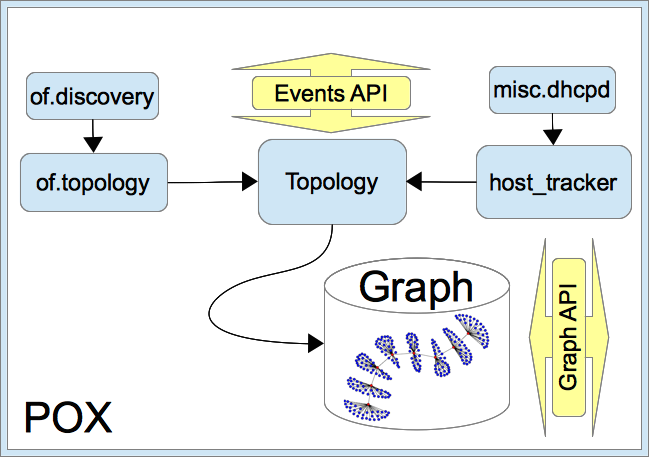
\includegraphics[scale=1.7]{img/design.png}
    \end{figure}
\end{frame}




%
% Experiments - Entity detection
%
\begin{frame}\frametitle{Entity detection}

    Performed by the \emph{topology} module
    \begin{itemize}
        \setlength{\itemsep}{10pt}
        \item Gets notifications from \emph{host\_tracker} and
            \emph{of.topology}
        \item Builds an event channel for updates
            \begin{itemize}
                \item join/leave events
                \item Other controller applications can listen to events they
                    care about
                \item Publisher/subscriber approach
            \end{itemize}
        \item Notifies join and leave of:
            \begin{itemize}
                \item Controller
                \item Switch
                \item Port
                \item Link
                \item Host
            \end{itemize}
    \end{itemize}
\end{frame}

%
% Experiments - Switches and Links
%
\begin{frame}\frametitle{Network devices detection}
    
    Performed by POX \emph{of.topology} module
    \begin{itemize}
        \item Uses LLDP to identify switches (POX's discovery class)
        \item Control informations about switches, links and ports
        \item Other modules may be created for other technologies
    \end{itemize}
\end{frame}


%
% Experiments - Host detection  
%
\begin{frame}\frametitle{Host detection}

    Performed by \emph{host\_tracker} module
    \begin{itemize}
        \item Listen to DHCP request/release messages
        \item Replaces ARP Protocol (answers to all requests)
    \end{itemize}
\end{frame}

\section{Experimentos}
\label{sec:experiments}

O objetivo dos experimentos é validar e avaliar o sistema proposto.
Considere-se uma rede com uma topologia simples conforme mostrado abaixo: 

\begin{figure}[h!]
    \centering
    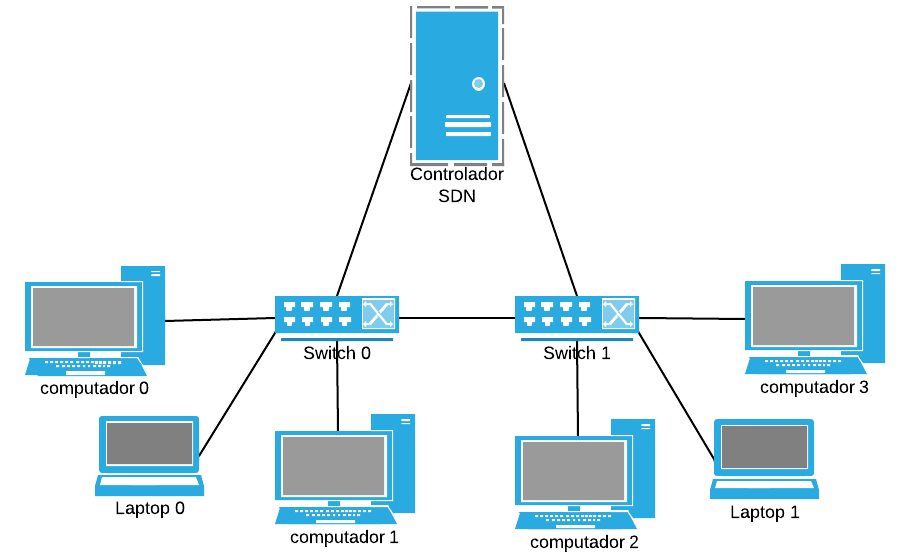
\includegraphics[scale=0.4]{mininet_topology.png}
    \caption{Topologia simples}
    \label{fig:topology}
\end{figure}

Conforme pode ser visto na figura \ref{fig:topology}, tem-se seis \emph{hosts} em sub-redes diferentes. 
Os dois \emph{switches} são controlados pela mesma instância do controlador 
POX.
Essa topologia foi configurada através do \emph{mininet} \citep{lantz2010network}. 
O mininet permite a criação de \emph{scripts} que geram topologias 
na rede simulada. 
Note que, na topologia proposta, existe um \emph{link} entre os dois 
switches.
Esse \emph{link} também é representado por uma aresta no modelo do grafo
proposto.


\subsection{Detecção de entidades}
O sistema inicia o grafo da rede vazio.
Os \emph{switches} são os primeiros a serem identificados. 
Como o controlador está ligado diretamente a eles pela interface 
\emph{OpenFlow}, um evento de \emph{ConnectionUp} é disparado 
pelo núcleo do controlador.

\begin{figure}[h!]
\centering
\begin{lstlisting}
INFO:topology.graph:SwitchJoin id: 2
INFO:topology.graph:SwitchJoin id: 1
INFO:topology.graph:1, 2
DEBUG:openflow.discovery:Dropping LLDP packet 275
INFO:topology.graph:LinkEvent fired
INFO:host_tracker:Learned 1 1 7e:e6:9b:89:39:2e got IP 10.0.0.1
INFO:topology.graph:HostJoin id: 7e:e6:9b:89:39:2e
INFO:host_tracker:Learned 2 1 62:77:44:24:13:49 got IP 10.0.0.2
INFO:topology.graph:HostJoin id: 62:77:44:24:13:49
\end{lstlisting}
\caption{Detecção de entidades}
\label{fig:detection}
\end{figure}

Nas duas primeiras linhas do \emph{log} mostrado na figura
\ref{fig:detection}, o módulo \emph{graph} foi notificado
da descoberta de dois \emph{switches} na rede.
A \emph{callback} do evento \emph{SwitchJoin} adiciona um vértice ao grafo. 
Assim, dois vértices do tipo \emph{switch} foram referenciados no grafo. 
Na linha 5, nota-se que a descoberta de um \emph{link} (entre switches).
O módulo \emph{openflow.discovery}, através do protocolo LLDP identificou 
o link entre \emph{switches}.
O grafo foi notificado e estabeleceu uma aresta entre os 
vértices (\emph{switches}).
As linhas 7 e 9 mostram a descoberta de dois hosts. 
Esses hosts foram descobertos pelo módulo \emph{host\_tracker} via 
escuta dos eventos de DHCP.
É importante ressaltar que a descoberta de \emph{hosts} também ocorre 
independente do DHCP.
Um novo pacote que passa por um \emph{switch} e não possui regra
instalada na tabela de fluxos é encaminhado ao controlador que 
dispara um evento de \emph{PacketIn}. 
Para tal, o \emph{host\_tracker} se encarrega de escutar esse evento 
e notificar o grafo através do evento \emph{HostJoin}.
O grafo, ao ser notificado, cria vértices para esses \emph{hosts} associando uma
aresta entre eles e o \emph{switch} ao qual eles estão conectados.
Dessa forma as entidades da rede são identificadas e computadas no grafo.

\subsection{Remoção de entidades}
Foram executados dois experimentos para validar a atualização do grafo
quando uma entidade (\emph{host/switch}) torna-se inativo/inalcançável.
Para o caso de remoção de \emph{host}, foi desligada a interface de 
rede de um \emph{host} via \emph{prompt} de comandos do mininet. 
O \emph{host\_tracker}, após um tempo fixo (\emph{timerInterval}) 
verifica via ARP Ping se os \emph{hosts} estão ativos.
Para esse cenário da remoção de um \emph{host}, após 30 segundos o 
\emph{host\_tracker} identificou a inatividade do \emph{host} e 
disparou o evento de \emph{HostLeave}, atualizando assim o grafo.
Para o caso do \emph{switch}, através do mininet, foi desligado um 
dos switches da topologia da figura \ref{fig:topology}.
O controlador está ligado diretamente ao \emph{switch}. 
Assim, ao ser desligado, o \emph{core} do POX dispara um evento 
de \emph{SwitchLeave} ao qual o módulo \emph{graph} está inscrito. 
Logo, o grafo é atualizado removendo o vértice do \emph{switch} e dos
\emph{hosts} ligados a ele. 

\subsection{Visualização em tempo real da rede}
Na figura \ref{fig:full_graph} é apresentado parte do grafo de uma rede
com 8 \emph{switches}, cada um com 30 \emph{hosts} conectados totalizando
248 entidades na rede.
Esse grafo é atualizado em tempo real em função dos eventos de rede ocorridos 
dentro do controlador, como entrada e saída de entidades, volume de tráfego 
na rede entre outros citados nesta seção. 

\begin{figure}[h!]
    \centering
    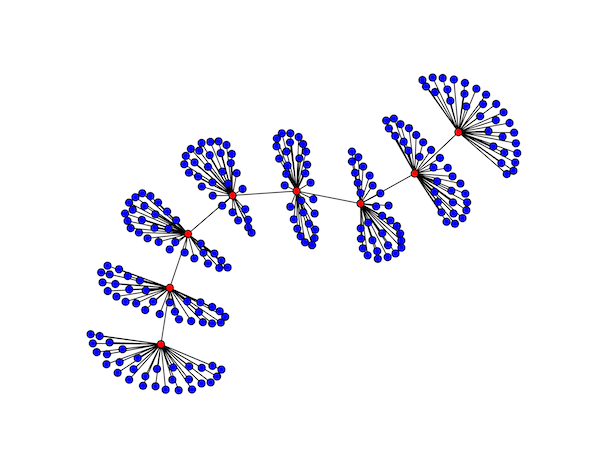
\includegraphics[scale=0.5]{full_graph.png}
    \caption{Grafo representando uma grande rede}
    \label{fig:full_graph}
\end{figure}

\subsection{Identificação de tráfego na rede}
Para computar o tráfego (TCP) na rede foi executado o programa \emph{iperf} 
como servidor no \emph{host} 'Host 0a' utilizando a topologia apresentada
na figura \ref{fig:topology}.
O \emph{host} 'Host 1e' conecta-se como cliente. 
Conformo pode ser notado na figura \ref{fig:iperf}, o tráfego 
em bytes na arestas desses \emph{hosts} é superior ao demais \emph{hosts}.
No momento em que foram lidos os contadores \emph{OpenFlow} e computados
os pesos das arestas, obteve-se um tráfego de 55894 bytes através do caminho
entre os dois \emph{hosts} citados.
Os valores apresentados para os demais \emph{hosts} (41 bytes) são referentes
ao tráfego ARP PING disseminado pelo módulo \emph{host\_tracker}
O experimento com o \emph{iperf} mostrou uma taxa de envio 
(\emph{throughput}) entre os \emph{hosts} de 300 Mega bits por segundo.

\begin{figure}[h!]
    \centering
    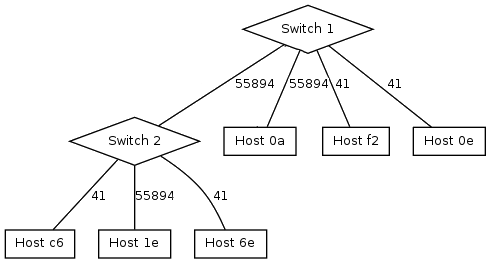
\includegraphics[scale=0.8]{graph_iperf.png}
    \caption{Tráfego TCP (em bytes) entre os hosts ’Host 1e’ e ’Host 0a’}
    \label{fig:iperf}
\end{figure}

\subsection{Árvore Geradora Mínima}
Uma árvore geradora mínima é mantida em tempo real sobre o grafo
da rede. 
Quando o grafo adiciona, remove ou atualiza arestas/vértices a árvore 
geradora mínima é computada. 
Outros módulos podem utilizá-la através da API do módulo em grafos.

Árvores geradoras mínimas são essenciais em diversas tarefas no gerenciamento
de redes.
Tarefas como disparar 'alarmes' quando a árvore estiver desconexa ou 
contenha \emph{loops}, conforme mostrado em \citep{schmid2013exploiting}.
É possível imaginar um sistema distribuído que consulte a árvore geradora
mínima para executar um algoritmo de propagação de mensagem \emph{flood} 
de maneira inteligente e menos custosa para 
a rede \citep{Monsanto:2013:CSN:2482626.2482629}.
Uma rede com múltiplos \emph{switches} pode implementar um 
balanceamento de carga eficiente que considere o tráfego nas arestas
utilizando a árvore geradora mínima em tempo real.
Além disso, é possível imaginar soluções como o \emph{Green MST}, 
apresentado em \citep{prete2012energy}. 
Uma abordagem em SDN utilizando uma árvore geradora mínima 
para reduzir o consumo elétrico da rede utilizando métricas da 
camada de aplicação. 

\section{Future work}
\label{sec:future}

As a future work we plan to build an on-line graph visualizer 
that interacts with the network administrator and shows, in 
an easier way, the entire network operation.
Just like POX, if the controller process is terminated, then the
entire graph is lost.
For that, a distributed graph database can be used to store
the network graph in a persistent, reliable and fault tolerant
structure.
Default graph algorithms should be given by the graph module. 
These algorithms could be configured to run in predefined 
period.
\section{Questions}

\begin{frame}
  {Questions?}

\begin{figure}[h]\vspace*{-1cm}
    \centering
    
\includegraphics[scale=0.3,width=\linewidth]{img/questions}
\end{figure}

Contatos:

\begin{itemize}
\item email: \href{mailto:gustavopantuza@gmail.com}{gustavopantuza@gmail.com}
\item github: \href{http://github.com/pantuza}{pantuza}
\item twitter: \href{http://twitter.com/gpantuza}{@gpantuza}
\item site: \href{http://pantuza.com}{http://pantuza.com}
\end{itemize}

\end{frame}



\end{document}
